% A one-page demo for the feedback reader. One sentence per line, so a click maps to one sentence.
% Try it:  latexmk -pdf -synctex=1 demo.tex  &&  ../bin/open-reader demo.pdf
\documentclass[11pt,a4paper]{article}
\usepackage[margin=2.5cm]{geometry}
\usepackage{amsmath}
\usepackage[version=4]{mhchem}
\usepackage{tikz}
\setlength{\parindent}{0pt}
\setlength{\parskip}{6pt}

\begin{document}

\section*{Machine-learned potentials for soft crystals}

Halide perovskites are soft, anharmonic crystals whose structure fluctuates strongly at room temperature.
Their atoms do not sit still at well-defined positions, so a single static structure is a poor description of the material.
Simulating these fluctuations directly with quantum-mechanical methods is accurate but far too slow for the length and time scales that matter.

Machine-learned interatomic potentials close this gap.
A model is trained on a few thousand quantum-mechanical calculations and then predicts energies and forces at a tiny fraction of the cost.
With such a model, molecular dynamics of thousands of atoms over nanoseconds becomes routine.

\begin{figure}[h]
	\centering
	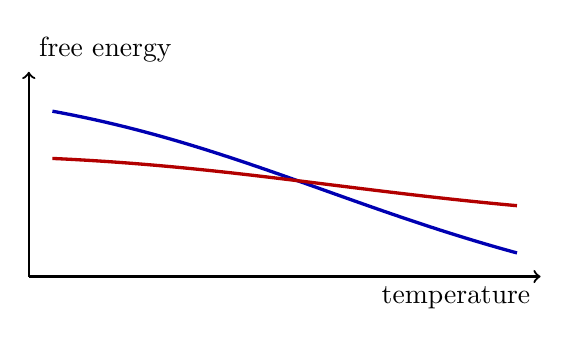
\begin{tikzpicture}
		\draw[thick,->] (0,0) -- (6.5,0) node[below left] {temperature};
		\draw[thick,->] (0,0) -- (0,2.6) node[above right] {free energy};
		\draw[very thick,blue!70!black] (0.3,2.1) .. controls (2.5,1.7) and (4,0.9) .. (6.2,0.3);
		\draw[very thick,red!70!black] (0.3,1.5) .. controls (2.5,1.4) and (4,1.1) .. (6.2,0.9);
	\end{tikzpicture}
	\caption{Free energy of two competing phases as a function of temperature, from thermodynamic integration.}
\end{figure}

The free energy of each phase follows from thermodynamic integration between a harmonic reference and the full anharmonic system,
\begin{equation}
	F(T) = F_\text{harm}(T) + \int_0^1 \langle U_1 - U_0 \rangle_\lambda \, \mathrm{d}\lambda .
\end{equation}
Comparing these free energies shows which phase is stable at each temperature, something static calculations at 0\,K cannot tell us.

\end{document}
